% !TEX program = pdflatex
% !TEX options = -synctex=1 -interaction=nonstopmode -file-line-error "%DOC%"
% Nonlinear Optics Assignment 2
\documentclass[UTF8,10pt,a4paper]{article}
\usepackage[scheme=plain]{ctex}
\newcommand{\CourseName}{Nonlinear Optics}
\newcommand{\CourseCode}{PHYS2202}
\newcommand{\Semester}{Spring, 2020}
\newcommand{\ProjectName}{Assignment 2}
\newcommand{\DueTimeType}{Due Time}
\newcommand{\DueTime}{13:00, March 17, 2020 (Tuesday)}
\newcommand{\StudentName}{陈稼霖}
\newcommand{\StudentID}{45875852}
\usepackage[vmargin=1in,hmargin=.5in]{geometry}
\usepackage{fancyhdr}
\usepackage{lastpage}
\usepackage{calc}
\pagestyle{fancy}
\fancyhf{}
\fancyhead[L]{\CourseName}
\fancyhead[C]{\ProjectName}
\fancyhead[R]{\StudentName}
\fancyfoot[R]{\thepage\ / \pageref{LastPage}}
\setlength\headheight{12pt}
\fancypagestyle{FirstPageStyle}{
    \fancyhf{}
    \fancyhead[L]{\CourseName\\
        \CourseCode\\
        \Semester}
    \fancyhead[C]{{\Huge\bfseries\ProjectName}\\
        \DueTimeType\ : \DueTime}
    \fancyhead[R]{Name : \makebox[\widthof{\StudentID}][s]{\StudentName}\\
        Student ID\@ : \StudentID\\
        Score : \underline{\makebox[\widthof{\StudentID}]{}}}
    \fancyfoot[R]{\thepage\ / \pageref{LastPage}}
    \setlength\headheight{36pt}
}
\usepackage{amsmath,amssymb,amsthm,bm}
\allowdisplaybreaks[4]
\newtheoremstyle{Problem}
{}
{}
{}
{}
{\bfseries}
{.}
{ }
{\thmname{#1}\thmnumber{ #2}\thmnote{ (#3)} Score: \underline{\qquad\qquad}}
\theoremstyle{Problem}
\newtheorem{prob}{Problem}
\newtheoremstyle{Solution}
{}
{}
{}
{}
{\bfseries}
{:}
{ }
{\thmname{#1}}
\makeatletter
\def\@endtheorem{\qed\endtrivlist\@endpefalse}
\makeatother
\theoremstyle{Solution}
\newtheorem*{sol}{Solution}
\usepackage{graphicx}
\begin{document}
\thispagestyle{FirstPageStyle}
\begin{prob}[Local field factors]
    We noted in lecture that for the general case of non-spherical symmetry, the local electric field, $\vec{E}^{(\text{loc})}$, can be written in terms of the macroscopic electric field, $\bm{E}$ and the polarization, $\vec{P}$ as
    \[
        \vec{E}^{\text{(loc)}}=\vec{E}+\frac{1}{\varepsilon_0}\overleftrightarrow{L}\cdot\vec{P}.
    \]
    (Note that the ppt handout has an error; $1/\varepsilon_0$ is replaced in the notes by $4\pi$, a relic from writing the equation in my notes in gaussian units rather than SI units.) We determined the value of $\overleftrightarrow{L}$ by a \textit{mean field} approximation in which we represent the medium, which in reality consists of discrete atomic or molecular units, by a continuous medium. If we assumed that the system has spherical symmetry (or more generally is isotropic), we were able to calculate that the tensor $\overleftrightarrow{L}$ reduces to $\overleftrightarrow{L}=L\bm{1}=\frac{1}{3}\bm{1}$ ($\bm{1}$ is the identity matrix). The local field factor is then the same in all directions and given by
    \[
        f(\omega)=1+(\varepsilon_r-1)L,
    \]
    where $\varepsilon_r$ is the relative permittivity.\\
    Given the dramatic implications of the local field factor in nonlinear optics, it is important to consider systems that are not isotropic. Indeed, in the case of anisotropic systems, the $\overleftrightarrow{L}$ takes different forms. (Fortunately, in the case of a linear relationship between the polarization and the local electric field, $\overleftrightarrow{L}$ can always be written in a diagonal form.) In general, for molecules with elongated or oblate shape, one can use ellipsoidal cavities with semiaxes $a_1$, $a_2$, $a_3$, and one finds that
    \[
        L_i=\frac{a_1a_2a_3}{2}\int_0^{\infty}\frac{1}{(s+a_i^2)\sqrt{(s+a_1^2)(s+a_2^2)(s+a_3^2)}}\,ds,
    \]
    which can be evaluated numerically.\\
    Here we will just investigate molecular crystals of closely packed molecules of simple symmetry.
    \begin{enumerate}
        \item[(a)] Suppose that the we are dealing with molecules that are rod-like (having a cylindrical form with radius $r$ much smaller than the length $l$).
        \begin{enumerate}
            \item[i.] Calculate the elements of the matrix $\overleftrightarrow{L}$.
            \item[ii.] To realize the largest local field factor, in what direction should the polarization of the electric field be?
            \item[iii.] What are the values of the largest and smallest local field factor if $\varepsilon_r=4$.
        \end{enumerate}
        \item[(b)] Answer the preceding questions for molecules that have a disk-like form (having a cylindrical form but with $r\gg l$).
        \item[(c)] Everything else being equal (for example, molecules that pack with the same number density), for what shape molecule (spherical, rod-like, or disk-like) do we expect to yield a molecular crystal with the largest local field factor?
    \end{enumerate}
\end{prob}
\begin{sol}
    \begin{enumerate}
        \item[(a)]
        \begin{enumerate}
            \item[(i.)] We first calculate $\overleftrightarrow{L}$ for molecules of general cylindrical form before considering the specific dimensions (the radius $r$ and length $l$) of the cylinder.

            Since the molecules are cylindrical, we assume that the molecule of interest is inside a micro cylindrical cavity within a continuous medium. To specify the orientation, we construct a rectangular coordinate whose origin is at the center of the cylindrical and $z$ axis is along the generatrix of the cylindrical, as shown in figure \ref{sketch}.\\
            \begin{figure}[h]
                \centering
                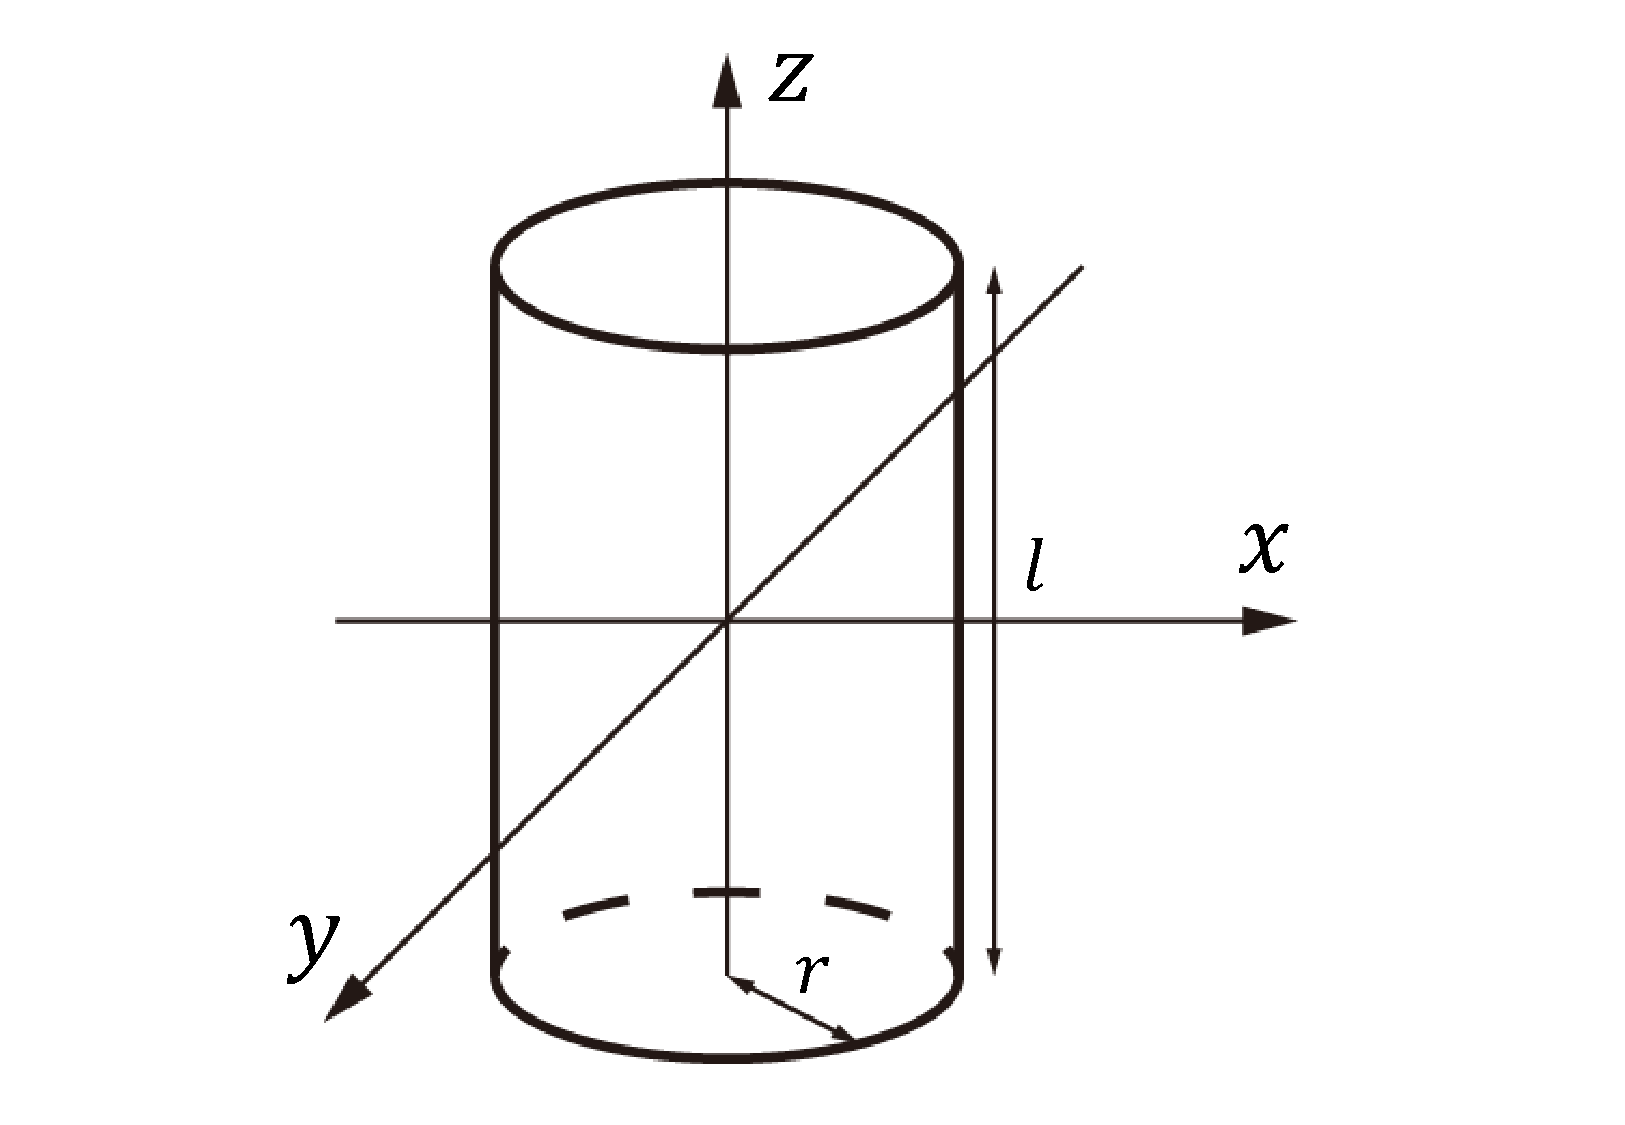
\includegraphics[width=.4\textwidth]{sketch.pdf}
                \caption{The cylinder cavity with the rectangular coordinate.}
                \label{sketch}
            \end{figure}

            As mentioned in the problem introduction, $\overleftrightarrow{L}$ can be written in a diagonal form in the case of linear relationship between the polarization and the local electric field, so we only need to calculate the three diagonal elements of $\overleftrightarrow{L}$: $L_{xx}$, $L_{yy}$, and $L_{zz}$ such that the component of the local electric field are express as
            \begin{gather}
                E_x^{(\text{loc})}=E_x+\frac{1}{\varepsilon_0}L_{xx}P_x,\\
                E_y^{\text{(loc)}}=E_y+\frac{1}{\varepsilon_0}L_{yy}P_y,\\
                E_z^{\text{(loc)}}=E_z+\frac{1}{\varepsilon_0}L_{zz}P_z.
            \end{gather}
            \begin{itemize}
                \item $L_{zz}$: If we apply an electric field that is along the positive direction of the $z$-axis, the density of the surface charge induced by the surrounding polarization medium is $\sigma=P$ (where $P$ is the polarization of the medium) on the bottom surface and $\sigma=-P$ on the top surface, but zero on the side surface. The field at the center of the cylindrical cavity generated by the surface charge is
                \begin{align}
                    \nonumber E^{(\text{cav})}=&2\cdot\frac{1}{4\pi\varepsilon_0}\int_{\text{top surface}}\frac{\sigma\cdot dS}{\tau^2+(l/2)^2}\cdot\frac{l/2}{\sqrt{\tau^2+(l/2)^2}}\\
                    \nonumber=&2\cdot\frac{1}{4\pi\varepsilon_0}\int_0^r\int_{-\pi}^{\pi}\frac{P\cdot \tau\,d\phi\,d\tau}{\tau^2+(l/2)^2}\cdot\frac{l/2}{\sqrt{\tau^2+(l/2)^2}}\\
                    \nonumber=&\frac{Pl}{4\pi\varepsilon_0}\int_0^r\frac{\tau\,d\tau}{(\tau^2+(l/2)^2)^{3/2}}\int_{-\pi}^{\pi}\,d\phi\\
                    \nonumber=&\frac{Pl}{4\pi\varepsilon_0}\cdot\left[-\frac{1}{\sqrt{r^2+(l/2)^2}}+\frac{2}{l}\right]\cdot 2\pi\\
                    =&\frac{Pl}{\varepsilon_0}\left(-\frac{1}{\sqrt{4r^2+l^2}}+\frac{1}{l}\right)
                \end{align}
                (some variables are denoted in figure \ref{sketch1}.)\\
                Considering
                \begin{equation}
                    E_z^{(\text{loc})}=E_z+E_z^{(\text{cav})}=E_z+\frac{1}{\varepsilon}L_{zz}P_z,
                \end{equation}
                we get the $zz$ component of $\overleftrightarrow{L}$:
                \begin{equation}
                    L_{zz}=l\left(-\frac{1}{\sqrt{4r^2+l^2}}+\frac{1}{l}\right).
                \end{equation}
                \begin{figure}[h]
                    \centering
                    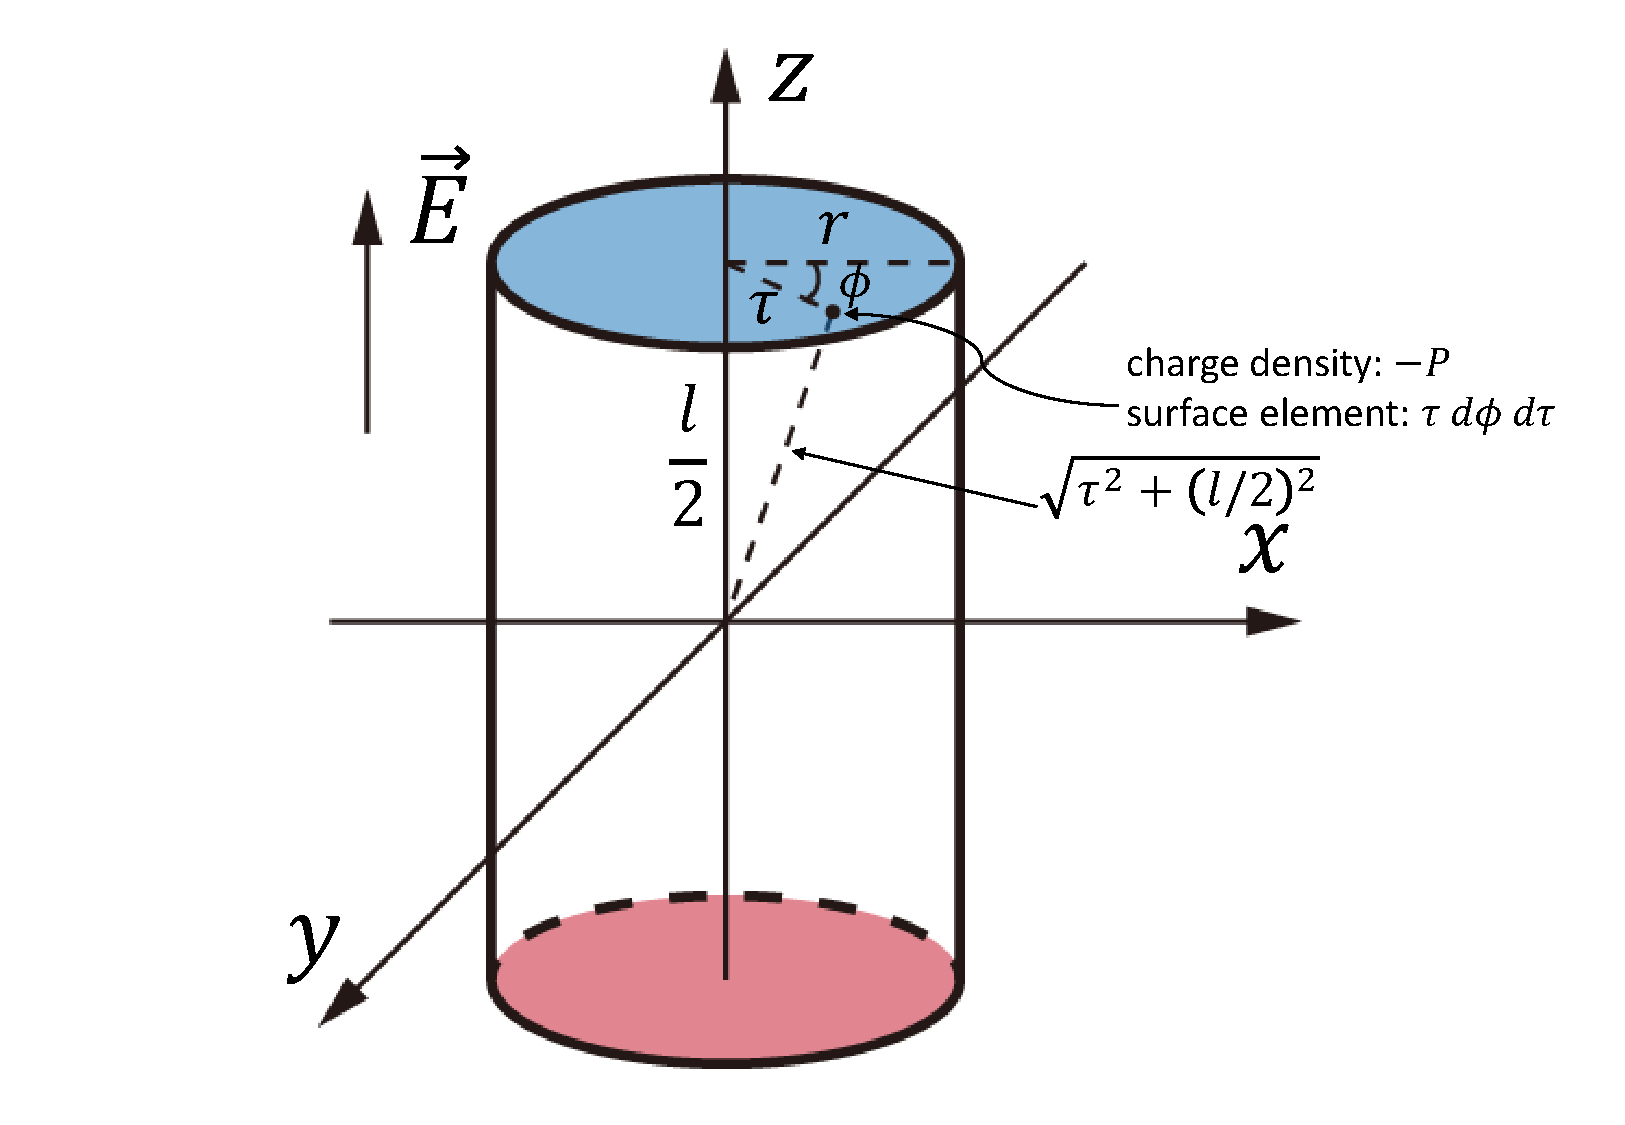
\includegraphics[width=.4\textwidth]{sketch1.pdf}
                    \caption{The surface charge distribution when applied with field along positive $z$ direction. Red filling represent the positive surface charge, blue represent negative.}
                    \label{sketch1}
                \end{figure}
                \item $L_{xx}$: If we apply the field along the positive $x$ direction, the induced surface charge density is $\sigma=P\cos\phi$ (where $\phi$ is the angle between the positive direction of the $x$-axis and the line connecting the interest point and the center of the cross-section where the interest point is on, as shown in figure \ref{sketch2}), while zero on the top and bottom surface. The electric field at the center of the cylindrical cavity generated by the surface charge is
                \begin{align}
                    \nonumber E^{(\text{cav})}=&2\cdot\frac{1}{4\pi\varepsilon_0}\iint_{\text{half side surface}}\frac{\sigma\cdot dS}{z^2+r^2}\cdot\frac{r}{\sqrt{z^2+r^2}}\cdot\cos\phi\\
                    \nonumber=&2\cdot\frac{1}{4\pi\varepsilon_0}\int_{-l/2}^{l/2}\int_{-\pi/2}^{\pi/2}\frac{P\cos\phi\cdot r\,d\phi\,dz}{z^2+r^2}\cdot\frac{r}{\sqrt{z^2+r^2}}\cdot\cos\phi\\
                    \nonumber=&\frac{Pr^2}{2\pi\varepsilon_0}\int_{-l/2}^{l/2}\frac{dz}{(z^2+r^2)^{3/2}}\int_{-\pi/2}^{\pi/2}\cos^2\phi\,d\phi\\
                    \nonumber=&\frac{Pr^2}{2\pi\varepsilon_0}\cdot\frac{l}{r^2\sqrt{(l/2)^2+r^2}}\cdot\frac{\pi}{2}\\
                    =&\frac{Pl}{2\varepsilon_0\sqrt{l^2+4r^2}}
                \end{align}
                Considering
                \begin{equation}
                    E_x^{(\text{loc})}=E_x+E_x^{(\text{cav})}=E+\frac{1}{\varepsilon_0}L_{xx}P_x,
                \end{equation}
                we get the $xx$ component of $\overleftrightarrow{L}$:
                \begin{equation}
                    L_{xx}=\frac{l}{2\sqrt{l^2+4r^2}}.
                \end{equation}
                \begin{figure}[h]
                    \centering
                    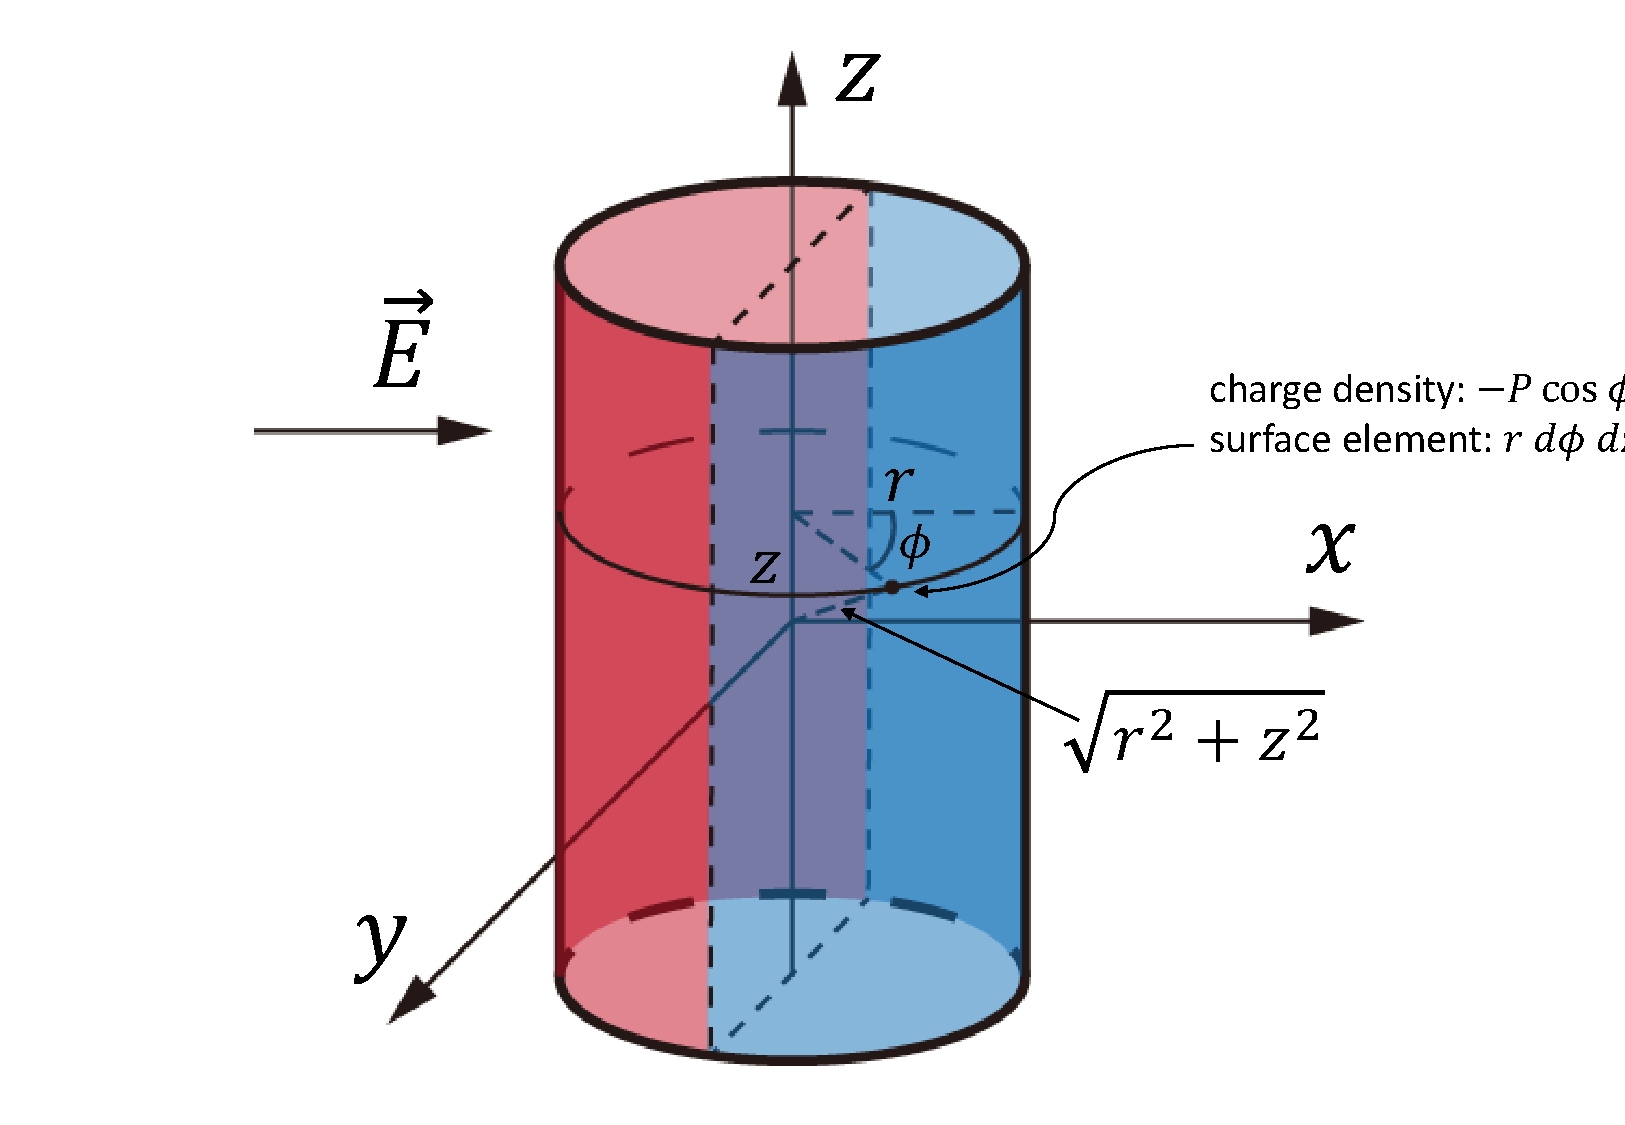
\includegraphics[width=.4\textwidth]{sketch2.pdf}
                    \caption{The surface charge distribution when applied with field along positive $x$ direction. Red filling represent the positive surface charge, blue represent negative.}
                    \label{sketch2}
                \end{figure}
                \item Due to the symmetry of the cylinder, the $yy$ component of $\overleftrightarrow{L}$ is the same as the $xx$ component:
                \begin{equation}
                    L_{yy}=L_{xx}=\frac{l}{2\sqrt{l^2+4r^2}}.
                \end{equation}
            \end{itemize}
            Now having the formula of the element of $\overleftrightarrow{L}$ for cylindrical molecules, we go back to the given limit condition: rod-like molecule. This implies that $r\ll l$, so we have
            \begin{gather}
                L_{zz}=\lim_{r\ll l}l\left(-\frac{1}{\sqrt{4r^2+l^2}}+\frac{1}{l}\right)=0,\\
                L_{xx}=L_{yy}=\lim_{r\ll l}\frac{l}{2\sqrt{l^2+4r^2}}=\frac{1}{2}.
            \end{gather}
            \item[(ii.)] Since the $xx$ and $yy$ component of $\overleftrightarrow{L}$ is greater than the $zz$ component, to realize the largest local field factor, the electric field should be perpendicular to the $z$-axis (or perpendicular to the generatrix) of the cylinder.
            \item[(iii.)] When the field is perpendicular to the $z$-axis, we have the largest local field factor:
            \begin{equation}
                f_{\max}=1+(\varepsilon_r-1)L_{xx/yy}=\frac{5}{2}.
            \end{equation}
            When the field is along the $x$-axis, we have the smallest local field factor:
            \begin{equation}
                f_{\min}=1+(\varepsilon_r-1)L_{zz}=1.
            \end{equation}
        \end{enumerate}
        \item[(b)] For disk-like molecules, the limit condition becomes $r\gg l$, so we have
        \begin{gather}
            L_{zz}=\lim_{r\gg l}l\left(-\frac{1}{\sqrt{4r^2+l^2}}+\frac{1}{l}\right)=1,\\
            L_{xx}=L_{yy}=\lim_{r\gg l}\frac{l}{2\sqrt{l^2+4r^2}}=0.
        \end{gather}

        Since the $zz$ component of $\overleftrightarrow{L}$ is greater than the $xx$ and $yy$ component, to realize the largest local field factor, the electric field should be along the $z$-axis (or along the generatrix) of the cylinder.

        When the field is along the $z$-axis, we have the largest local field factor:
        \begin{equation}
            f_{\max}=1+(\varepsilon_r-1)L_{zz}=4.
        \end{equation}
        When the field is perpendicular to the $z$-axis, we have the smallest local field factor:
        \begin{equation}
            f_{\min}=1+(\varepsilon_r-1)L_{xx/yy}=1.
        \end{equation}
        \item[(c)] For spherical molecule with the same $\varepsilon_r=4$, its local field factor is
        \begin{equation}
            f=1+(\varepsilon_r-1)L=2.
        \end{equation}
        Therefore, the \textbf{disk-like} molecule can yield a molecular crystal with the largest local field factor.
    \end{enumerate}
\end{sol}
\end{document}